% ============================================================================
%  Short paper -- Hanoi urban noise, low-cost protocol + agent-based exposure
%
%  Self-contained. Compiles with pdflatex + bibtex, no exotic packages:
%      pdflatex main && bibtex main && pdflatex main && pdflatex main
%  Ready to zip (main.tex, refs.bib, figures/) and upload to Overleaf.
%
%  TARGET VENUE: not yet fixed. The layout below is a neutral two-column A4
%  article; if the
%  target turns out to be an ACM venue, replace the \documentclass line with
%  \documentclass[sigconf,anonymous=false]{acmart} and delete the geometry,
%  fancyhdr and titling settings -- the body text needs no other change.
%
%  NO NUMBER IN THIS FILE IS TYPED FROM MEMORY. Every figure quoted is traceable
%  to models/metrics.json or to a named script in the repository.
% ============================================================================
\documentclass[10pt,twocolumn,a4paper]{article}

\usepackage[T1]{fontenc}
\usepackage[utf8]{inputenc}
\usepackage[english]{babel}
\usepackage{lmodern}
\usepackage{microtype}
\usepackage[margin=18mm,columnsep=6mm]{geometry}
\usepackage{booktabs}
\usepackage{graphicx}
\usepackage{amsmath}
\usepackage{caption}
\usepackage{enumitem}
\usepackage{xcolor}
\usepackage[round,authoryear]{natbib}
\usepackage[hidelinks]{hyperref}

\graphicspath{{figures/}}
\captionsetup{font=small, labelfont=bf, skip=4pt}
\setlist{itemsep=.2em, topsep=.3em, parsep=0pt, leftmargin=1.2em}
\renewcommand{\arraystretch}{1.12}
\emergencystretch=2em

\definecolor{warnc}{HTML}{8A4B08}
\newcommand{\LAt}{$L_{A,25\mathrm{s}}$}
\newcommand{\dB}{\ensuremath{\,\mathrm{dB}}}

\title{\vspace{-1.2em}\bfseries What a smartphone protocol can establish about
urban noise:\\ three negative results and an agent-based exposure model for Hanoi
\vspace{-.4em}}

\author{%
  Laurian Jamin \and Lucas Zborowski\\[.2em]
  {\small ISIMA, Clermont-Ferrand, France, COSMOS Lab, VinUniversity, Hanoi}\\
  {\small\texttt{laurian@laurian-jamin.fr}}
  \vspace{-1em}}
\date{}

\begin{document}
\maketitle

\begin{abstract}\small\noindent
Hanoi is dense, motorcycle-dominated and has no routine noise monitoring, and
professional instrumentation is out of reach of most local budgets. We report
what a noise-mapping protocol built from three consumer smartphones and open
data does and does not establish, over 363 field measurements taken across three
contrasted urban typologies between 10~June and 22~July~2026. Evaluated under
three cross-validation protocols of increasing severity, with a
2\,000-replicate block bootstrap, our results are three negative ones.
\textbf{(i)} A three-parameter line-source attenuation kernel outperforms every
learned model we built, including a physics-plus-residual hybrid we had
ourselves recommended: the ranking of seven models \emph{inverts} between a
permissive spatial split and two strict ones. \textbf{(ii)} Cross-city transfer
from a 61\,000-point Ugandan corpus fails, not by an offset, but by carrying
no usable information at all, while one locally fitted distance term reaches
$R^2 = 0.240$. \textbf{(iii)} Vehicle counts extracted from 147 matched traffic
videos yield exactly zero emission coefficients for motorcycles and cars, as
density and as line-crossing flow alike. We deliver the surviving model as a
40\,m exposure map driving an agent-based simulation in which \emph{receiver}
agents, not emitter agents, accumulate a noise dose, a design forced by the
absence of any per-street data that emitter agents could be calibrated or
verified against.
\end{abstract}

\vspace{.4em}

% ============================================================================
\section{Introduction}

Vietnam has no national strategic noise mapping programme and no statutory noise
action plan \citep{nguyen2025law}, and class~1 or class~2 sound level meters and
commercial propagation software sit outside most local research budgets. This is
exactly the setting in which low-cost participatory noise mapping is proposed. It
is also a setting in which the claims such a method can support are rarely
tested.

We ran a three-month campaign in Hanoi and then evaluated it adversarially. Our
contribution is not a noise map of Hanoi, our instrument cannot support one, but a set of \textbf{boundary conditions on low-cost urban noise modelling},
each obtained from an experiment designed to succeed.

The agent-based component is where the constraint bites hardest and is, we
believe, of independent interest: with no per-street flows, no modal shares, no
speeds and no signal cycles, an emitter-agent traffic simulation would be neither
calibratable nor verifiable. We therefore invert the usual construction and put
the agents on the \emph{receiving} side of a measured field.

% ============================================================================
\section{Data and protocol}

363 measurements were collected across three deliberately contrasted typologies
, a new peri-urban development (Ocean Park, $n=184$), a historic dense quarter
(Hoan Kiem lake, $n=99$) and a transport corridor (Vinh Tuy, $n=80$), using
ODK~Collect against a KoboToolbox server, with a 10\,m GPS accuracy gate and a
recorded outdoor distance to the road. 147 timestamped traffic videos were
recorded alongside (median video-to-measurement offset 15\,s).

\paragraph{The quantity, stated precisely.} Each record is one A-weighted,
SLOW-weighted level over a 20--30\,s stationary observation, which we denote
\LAt{} and never $L_{A\mathrm{eq}}$, $L_\mathrm{den}$ or $L_\mathrm{night}$. The three handsets
were cross-calibrated \emph{against one another} and against no standard, so a
bias common to all three is invisible in the data by construction. Consumer
smartphone measurement is known to depart from reference instruments by several
decibels in a handset-, OS- and level-dependent way that is not a constant offset
\citep{kardous2014smartphone, murphy2016smartphone}. Accordingly:

\begin{itemize}
  \item contrasts between places, hours and typologies are supported, because a
        common bias cancels in a difference;
  \item absolute levels are reported with a bounded bias interval
        (+3.0 to +7.3\dB) estimated against instrumented Vietnamese campaigns
        \citep{phan2010characteristics, gelb2019cyclists} and never applied;
  \item \textbf{no compliance claim is made.} QCVN~26:2010 \citep{qcvn26}
        thresholds appear only as descriptive colour bands. A WHO
        $L_\mathrm{den}$/$L_\mathrm{night}$ comparison present in an earlier
        version of this work was withdrawn in full.
\end{itemize}

\begin{figure}[t]
  \centering
  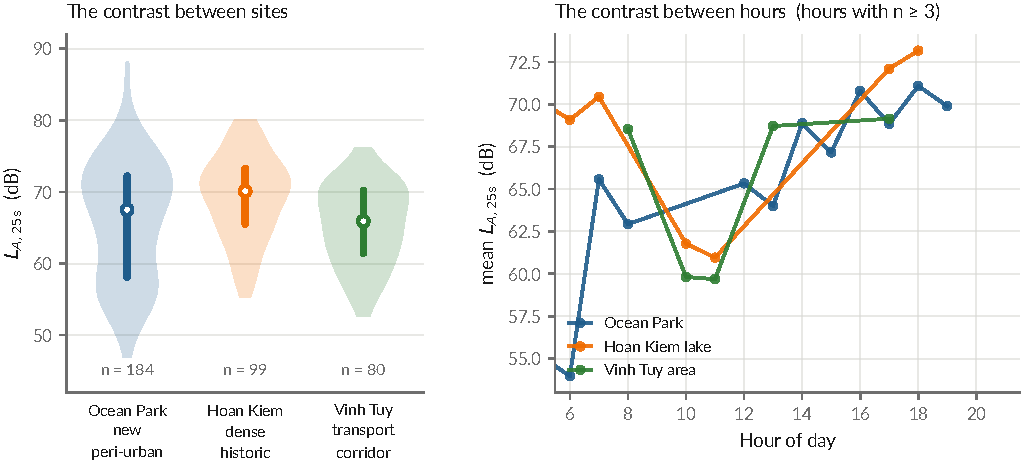
\includegraphics[width=.96\columnwidth]{campaign.pdf}
  \caption{The 363 measurements: spatial layout, level distribution and temporal
  coverage across the three typologies.}
  \label{fig:campaign}
\end{figure}

% ============================================================================
\section{Evaluation framework}

Eight models are scored on \emph{identical folds} under three protocols of
increasing severity: 600\,m spatial block cross-validation (17 blocks); buffered
leave-one-out with a 300\,m exclusion radius; and leave-one-site-out. Confidence
intervals come from a 2\,000-replicate block bootstrap.

The middle protocol is our \textbf{reference}, because its exclusion radius
equals the radius over which the morphological features are aggregated. This is
not a detail. An earlier version of this work reported $R^2 = 0.45$ under a
grouping on $\sim$110\,m cells, smaller than the 300\,m feature radius; that
protocol leaked between folds \citep{roberts2017crossvalidation} and the figure
was withdrawn. The delivered model is now selected \emph{by code}, best score
under the reference protocol among candidates fixed in advance, so that a
published map cannot silently inherit a model that only wins on a permissive
split.

% ============================================================================
\section{Result 1: geometry beats learning}

The delivered model treats each road class as an incoherent line source, whose
intensity falls as $1/d$ rather than $1/d^{2}$:
\[
E(x) = \frac{A_{\mathrm{hw}}}{\max(d_{\mathrm{hw}}, d_0)}
     + \frac{A_{\mathrm{res}}}{\max(d_{\mathrm{res}}, d_0)} + B,
\]
$L(x) = 10\log_{10}E(x)$, with $d_{\mathrm{hw}}$ and $d_{\mathrm{res}}$ the
distances to the nearest major axis and to the nearest local street, separated by
OSM \texttt{highway} tag, three non-negative coefficients and $d_0 = 5$\,m.

\begin{table}[t]\centering\footnotesize
\caption{$R^2$ under the three protocols, 95\,\% block-bootstrap intervals,
$n=363$. Reference protocol in the middle column. Best per column in bold.}
\label{tab:models}
\begin{tabular}{@{}lccc@{}}
\toprule
\textbf{Model} & \textbf{Block-CV} & \textbf{Buff.\ LOO} & \textbf{LOSO} \\
 & 600\,m & 300\,m & \\
\midrule
Mean by (site, hour)      & $-0.008$ & $-0.419$ & $-0.058$ \\
$\log d_{\text{road}}$ (2 par.) & 0.221 & 0.200 & 0.189 \\
\textbf{Physical (3 par.)} & 0.255 & \textbf{0.246} & \textbf{0.222} \\
LightGBM v1 (6 feat.)     & 0.304 & 0.137 & 0.029 \\
LightGBM v2 (8 feat.)     & 0.332 & 0.099 & $-0.035$ \\
Hybrid (physics + ML)     & \textbf{0.395} & 0.123 & 0.035 \\
Hybrid, restricted        & 0.378 & 0.144 & 0.106 \\
\bottomrule
\end{tabular}
\end{table}

\begin{figure}[t]
  \centering
  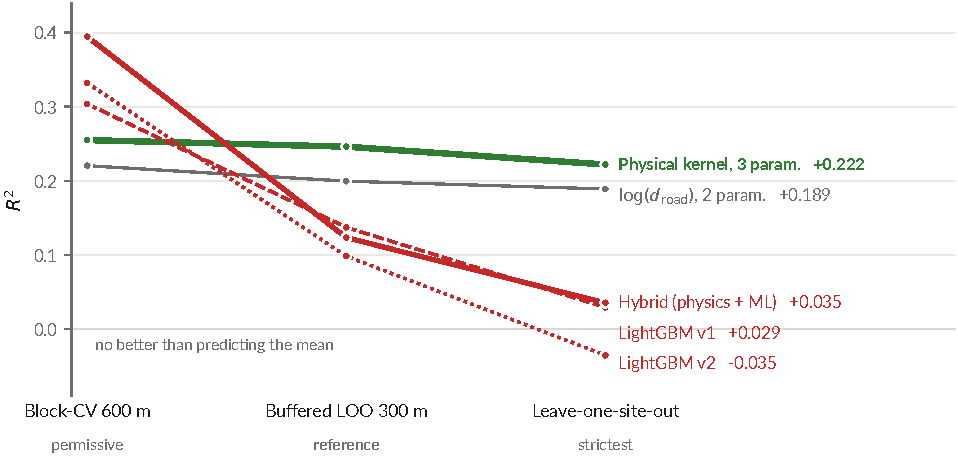
\includegraphics[width=.96\columnwidth]{ranking-inversion.pdf}
  \caption{The inversion. Same models, same folds; the ordering reverses almost
  exactly as the split begins to test generalisation.}
  \label{fig:inversion}
\end{figure}

\textbf{Read Table~\ref{tab:models} by column and the ranking reverses}
(Fig.~\ref{fig:inversion}). Every elaboration we added improves the permissive
protocol and degrades the strict ones, monotonically, the signature of
capacity fitting spatial autocorrelation rather than physics. Three readings
follow.

\emph{The morphological aggregates have negative marginal value.} Adding
built-area ratio, road density and intersection count to distance-to-road
degrades prediction by 0.07 $R^2$ under block-CV, 0.16 under buffered LOO and
0.18 under leave-one-site-out. A 300\,m disk is large enough to average away the
canyon geometry that governs propagation and small enough to be strongly
autocorrelated between neighbouring points: it supplies variance without
supplying information.

\emph{What survives in the learned model is time, not space.} The gap between the
full model and the morphology-only ablation under block-CV (0.304 vs 0.153) is
carried by hour-of-day. Under leave-one-site-out the time-only ablation is itself
negative ($-0.139$): it does not help predict an unmeasured location, which is
what a map is for.

\emph{The hybrid was built and rejected, not deferred.} We proposed the
physics-plus-learned-residual architecture ourselves as the constructive answer
to our own negative results. Built and evaluated on identical folds, the residual
gains $\Delta R^2 = +0.140$ under block-CV and loses $-0.123$ and $-0.187$ under
the two strict protocols. Constraining its capacity recovers part of the loss, and the direction of that trade is the diagnosis: what the unconstrained residual
learns is the spatial arrangement of our points, not physics the core is missing.
The residual is computed at every run and deliberately not applied.

\paragraph{A ceiling, so that $R^2 = 0.25$ can be read.} Two measurements within
40\,m of each other \emph{at the same hour} must be predicted identically by any
spatial model, so their disagreement is variance no spatial model can explain.
Over 87 such pairs the mean absolute difference is 5.44\dB, implying
$\sigma \approx 4.8$\dB{} against a total variance of 51\dB$^2$, a ceiling
near $R^2 \approx 0.54$. The delivered model reaches about half of what is
attainable, not a tenth of it. (Pairs at the same hour may fall on different
days, so this $\sigma$ carries day-to-day variation: it is an order of magnitude,
not a bound.)

\begin{figure}[t]
  \centering
  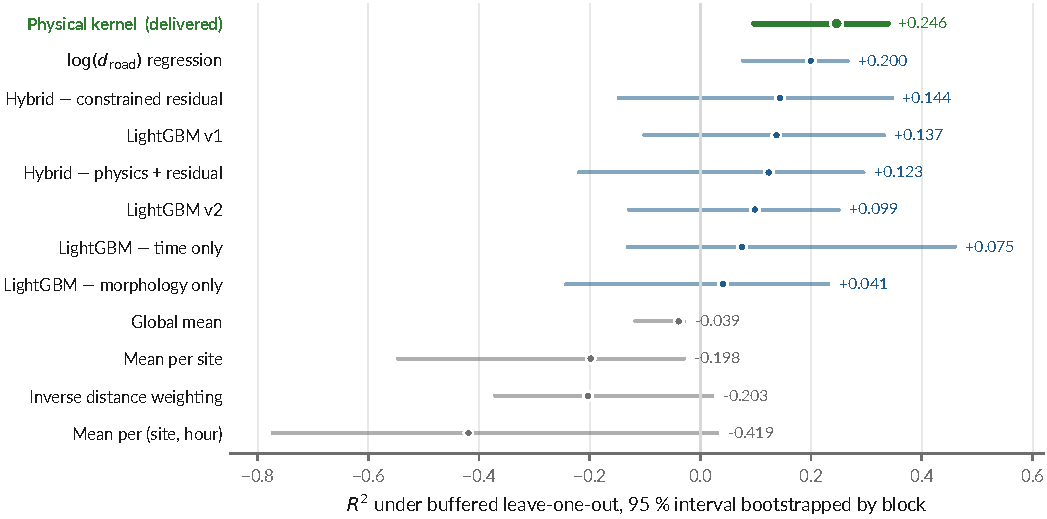
\includegraphics[width=.96\columnwidth]{forest-bloo.pdf}
  \caption{Every model under the reference protocol with its 95\,\% interval. The
  physical kernel is the only model whose interval excludes zero under all three
  protocols, and it is not separated from the two-parameter distance
  regression.}
  \label{fig:forest}
\end{figure}

% ============================================================================
\section{Result 2: transfer fails, and not by an offset}

Following the methodology we reproduce \citep{nsumba2026sunbird}, we pretrained a
morphology-to-level model on the Uganda 61K corpus and applied it to Hanoi. The
feature set was deliberately reformulated to be invariant to OSM mapping
conventions after a first version proved sensitive to them (Kampala is mapped as
individual buildings, Barcelona as whole blocks).

\begin{table}[t]\centering\footnotesize
\caption{Uganda-pretrained models evaluated on the 363 Hanoi points. Re-run
24~August 2026 from the versioned boosters.}
\label{tab:transfer}
\begin{tabular}{@{}lcccc@{}}
\toprule
 & as & mean diff. & rescaled & \\
\textbf{Pretrained} & delivered & removed & ($=r^2$) & $r$ \\
\midrule
Uganda 61K (v1)   & $-15.86$ & $-2.14$ & $+0.141$ & $-0.376$ \\
Uganda inv.\ (v2) & $-8.17$  & $-0.95$ & $+0.006$ & $+0.076$ \\
\midrule
\multicolumn{5}{@{}l}{\emph{Fitted locally on the same points:}}\\
$\log d_{\text{road}}$ & \multicolumn{4}{l}{$R^2 = +0.240$ (in sample)}\\
Physical, buff.\ LOO   & \multicolumn{4}{l}{$R^2 = +0.246$}\\
\bottomrule
\end{tabular}
\end{table}

Three readings of Table~\ref{tab:transfer}, and the third is the one that
matters. \textbf{It is not a calibration offset}: the Kampala model predicts
about 26\dB{} below Hanoi, and removing that difference leaves $R^2$ negative, so
a recalibrated transfer would not work either. \textbf{v1 transfers
anti-information}: its correlation with Hanoi is negative, it ranks quiet and
loud the wrong way round. \textbf{v2 removes the convention artefact and leaves
nothing}: $r = +0.076$, and even granted a free bias and a free slope its ceiling
is $R^2 = 0.006$. Not wrong, empty.

Against which, one locally fitted distance term on the same 363 points reaches
$R^2 = 0.240$. \textbf{Local measurement is not a refinement of transfer; it is a
prerequisite.} We attribute the failure to fleet composition and horn behaviour
\citep{nguyen2025horn}, to the same morphological descriptor denoting different
urban forms in different cities, and to target quantities that are not
exchangeable across studies.

% ============================================================================
\section{Result 3: video counts carry no acoustic signal}

Regressing measured acoustic \emph{energy} on vehicle counts,
$E = E_{\mathrm{bg}(s)} + \sum_c n_c e_c$ with $e_c \ge 0$, returns exactly zero
for motorcycles and cars. When we traced this to the choice of quantity, a
per-frame count is a \emph{stock}, while emission is driven by \emph{flow}, and
the two decouple exactly in congestion, we implemented our own recommendation,
re-processing all 147 videos with multi-object tracking and line-crossing counts.

\textbf{Flow does not rescue it.} Pooled, total flow against level gives
$r = -0.109$ and motorcycle flow $r = -0.004$. The two obstacles we did not
remove are the explanation: speed is unobservable without a ground homography and
dominates emission above 30--40\,km/h
\citep{kephalopoulos2014cnossos}, and distance is discarded because the field of
view is not georeferenced.

\begin{quote}\small
Instrument for $(Q, v)$ \emph{and} georeference the field of view. Obtaining $Q$
alone buys a coherent traffic statistic and no acoustic calibration.
\end{quote}

\noindent\textbf{We state a caveat on our own negative result.} Our detector was
never validated against manual counts, and it returns a modal split of 57\,\%
cars against 36\,\% motorcycles, in Hanoi, where reality is roughly the
inverse. This result should therefore be read as \emph{``the chain could not be
made to work''} rather than as a finding about acoustics.

% ============================================================================
\section{Receiver agents over a measured field}

\begin{figure}[t]
  \centering
  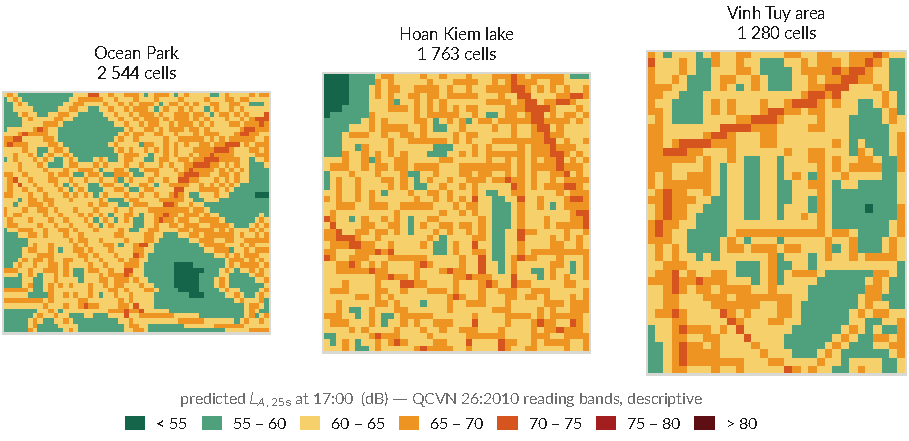
\includegraphics[width=\columnwidth]{map-grid.pdf}
  \caption{The delivered 40\,m grid, 5\,587 cells over three zones $\times$ 17
  hours, restricted to the sampled envelope (three sites plus 400\,m). Colour
  bands are QCVN~26:2010 references, shown descriptively.}
  \label{fig:grid}
\end{figure}

The surviving model is exported as a 40\,m grid (Fig.~\ref{fig:grid}) and drives
an agent-based simulation in GAMA. The design decision is the paper's fourth
contribution, and it is a negative one applied constructively.

\textbf{Emitter agents were rejected.} Motorcycle and car agents need real
per-street flows, fleet composition, speeds and signal cycles. We have none of
these for Hanoi, Result~3 is precisely the failure of our attempt to recover
them, so an emitter simulation would be neither calibratable against data nor
verifiable against anything.

\textbf{Receiver agents were adopted.} Agents move through the area and
accumulate a \emph{noise dose}: the level of the cell crossed, times the time
spent in it. The input is a map that was measured and validated; nothing about
the sources is invented. What emerges at population level, the distribution of
daily exposure, is what a map alone cannot give.

Against 360 matched measurement points the simulated field has mean error
$-1.24$\dB, MAE 5.30\dB{} and RMSE 6.49\dB. It reproduces the spatial and
temporal ordering and does not reproduce the spread, which is expected: features
aggregated over 300\,m cannot resolve a facade/courtyard contrast. One correction
is worth recording, because it is easy to get wrong, the traffic multiplier
must scale the \emph{traffic share} of the energy and never the background;
applied to total energy it double-counts the background and inflated the apparent
benefit of pedestrianisation from 3.5\dB{} to 7.0\dB.

Mobile receiver agents with daily journeys (``tier~2'') are specified and
\textbf{not yet implemented}; they are the natural next increment.

% ============================================================================
\section{Limitations}

Two limitations are not fixable by code and bound everything above. \textbf{There
is no absolute reference}: three handsets cross-calibrated against each other and
against no standard. \textbf{Three sites are three typologies}, the effective
number of independent morphological configurations is close to three whatever the
number of points, and three is not a basis for claiming coverage of a city. In
line with area-of-applicability reasoning \citep{meyer2021aoa} we therefore
restrict every published map to the sampled envelope, irrespective of score, and
we withdrew an earlier map covering a district in which nothing was measured.

Three further limits are open: the headline ranking is not statistically
separated (physical $0.246\,[0.097, 0.339]$ against $\log d_{\text{road}}$
$0.200\,[0.077, 0.266]$, Fig.~\ref{fig:forest}); the vehicle detector is
unvalidated; and a $-5$\dB{} discontinuity in the level distribution on
27~June~2026, coinciding with a change of form version, is spatially structured
and has no term in any of our models; it is not diagnosed here.

% ============================================================================
\section{Conclusion and future work}

At our sampling density and typological coverage, the predictable part of the
spatial variation in urban noise is the geometric divergence of sound from the
road network. A three-parameter line-source model captures it more robustly than
any learned model we built, including a hybrid using that same model as its base;
morphology aggregated over 300\,m adds no measurable value under any protocol.
We recommend that a distance-to-source physical baseline be reported as a
mandatory reference in every morphology-based noise mapping study, under a
spatial split whose block size exceeds the feature aggregation radius.

The indicated continuation is a real propagation kernel, CNOSSOS-EU via
NoiseModelling \citep{kephalopoulos2014cnossos, bocher2019noisemodelling}, which models what a distance law cannot: diffraction around buildings and
first- and second-order reflections. If a two-parameter distance term already
beats a six-variable gradient-boosting model, a physical propagation core
corrected by a locally learned residual is the architecture the data points at.

\paragraph{Data and code availability.} The 363 measurements, the 147 video
counts, the survey forms, the full pipeline, the GAMA model and the evaluation
framework are released at
\url{https://github.com/Colauz/noise-modelling-hanoi} (code MIT, data CC-BY-4.0).
Traffic videos and raw survey exports are not distributed, for the reasons stated
there.

\paragraph{Acknowledgements.} This work was carried out at COSMOS Lab,
VinUniversity, Hanoi, under the supervision of Doanh Nguyen-Ngoc. We thank
Nguyen Thanh Quang (VinUniversity) for his contribution to the field campaign
and for running the distribution of the field application.

\scriptsize
\setlength{\bibsep}{2pt plus 1pt}
\bibliographystyle{plainnat}
\bibliography{refs}

\end{document}
